\documentclass{article}
\usepackage[margin=1in]{geometry}
\usepackage{longtable,graphicx}
\begin{document}
\section*{Six-flow source recovery evaluation}
PASS means no reproducible final divergence was detected within the recorded valid inputs and budget; it is not a universal equivalence proof.
\begin{longtable}{llllllllllllllll}
Flow & N & Eligible N & First-pass RSR & Final RSR@R & Program Behavioral Pass Rate & Initial Behavioral Pass Rate & Final Behavioral Pass Rate & Input Match Macro & Input Match Micro & Counterexample Detection Rate & Canonical E2E & Compilation Repair Gain & Behavioral Repair Gain & Mean Tokens & Mean Runtime \\ \hline
F1 & 40 & 40 & 37/38 (97.4\%) & 38/38 (100.0\%) & 31/38 (81.6\%) & 21/38 (55.3\%) & 31/38 (81.6\%) & 87.8\% & 92.0\% & 7/38 (18.4\%) & 31/40 (77.5\%) & +2.6 pp & +26.3 pp & 537965 & 220.7s \\
F2 & 40 & 31 & 30/30 (100.0\%) & 30/30 (100.0\%) & 21/30 (70.0\%) & 21/30 (70.0\%) & 21/30 (70.0\%) & 86.7\% & 92.4\% & 9/30 (30.0\%) & 21/31 (67.7\%) & N/A & N/A & 146770 & 67.7s \\
F3 & 40 & 40 & 40/40 (100.0\%) & 40/40 (100.0\%) & 32/40 (80.0\%) & 22/40 (55.0\%) & 32/40 (80.0\%) & 90.8\% & 93.5\% & 8/40 (20.0\%) & 32/40 (80.0\%) & +0.0 pp & +25.0 pp & 517928 & 201.0s \\
F4 & 40 & 40 & 40/40 (100.0\%) & 40/40 (100.0\%) & 32/40 (80.0\%) & 24/40 (60.0\%) & 32/40 (80.0\%) & 92.1\% & 96.4\% & 8/40 (20.0\%) & 32/40 (80.0\%) & +0.0 pp & +20.0 pp & 494691 & 175.1s \\
F5 & 40 & 40 & 36/37 (97.3\%) & 37/37 (100.0\%) & 25/37 (67.6\%) & 10/37 (27.0\%) & 25/37 (67.6\%) & 74.7\% & 77.1\% & 12/37 (32.4\%) & 25/40 (62.5\%) & +2.7 pp & +40.5 pp & 1328970 & 291.8s \\
F6 & 40 & 40 & 22/23 (95.7\%) & 22/23 (95.7\%) & 7/21 (33.3\%) & 7/21 (33.3\%) & 7/21 (33.3\%) & 54.1\% & 57.5\% & 14/21 (66.7\%) & 7/40 (17.5\%) & N/A & N/A & 368247 & N/A \\
\end{longtable}
\begin{figure}[p]\centering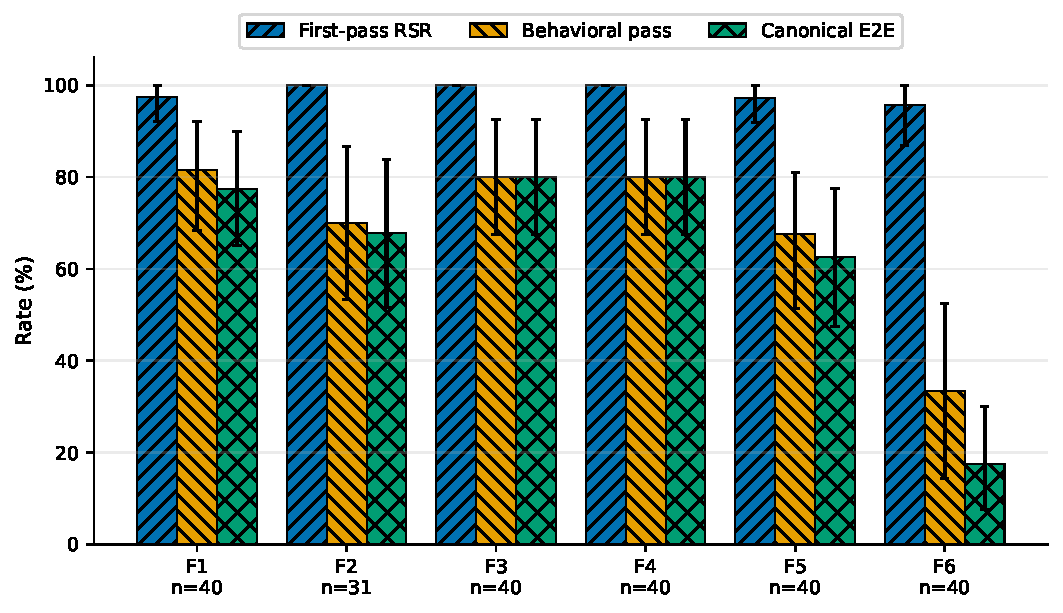
\includegraphics[width=.9\linewidth]{figures/overall_performance.pdf}\caption{Primary recovery outcomes with flow order F1–F6; F6 is derived from F5's first provider call.}\end{figure}
\begin{figure}[p]\centering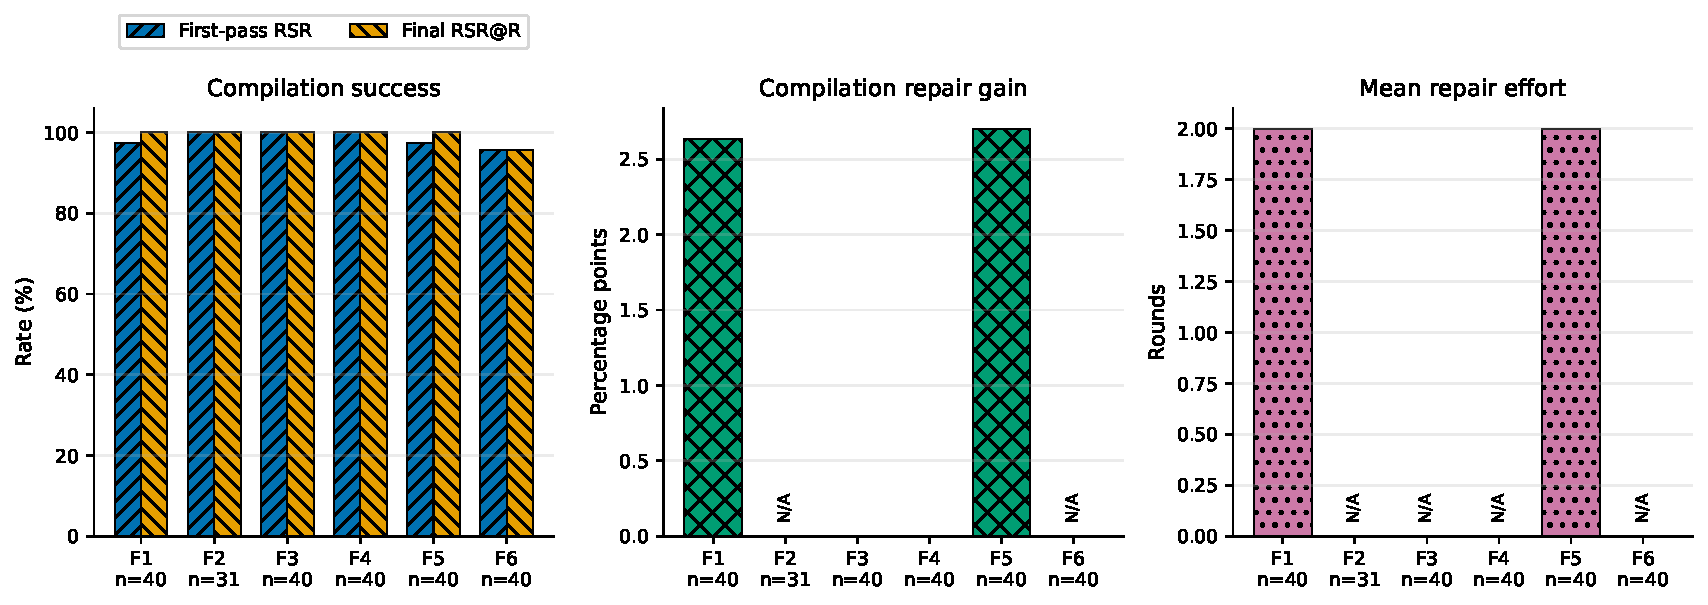
\includegraphics[width=.9\linewidth]{figures/compilation_performance.pdf}\caption{Compilation success before and after repair.}\end{figure}
\begin{figure}[p]\centering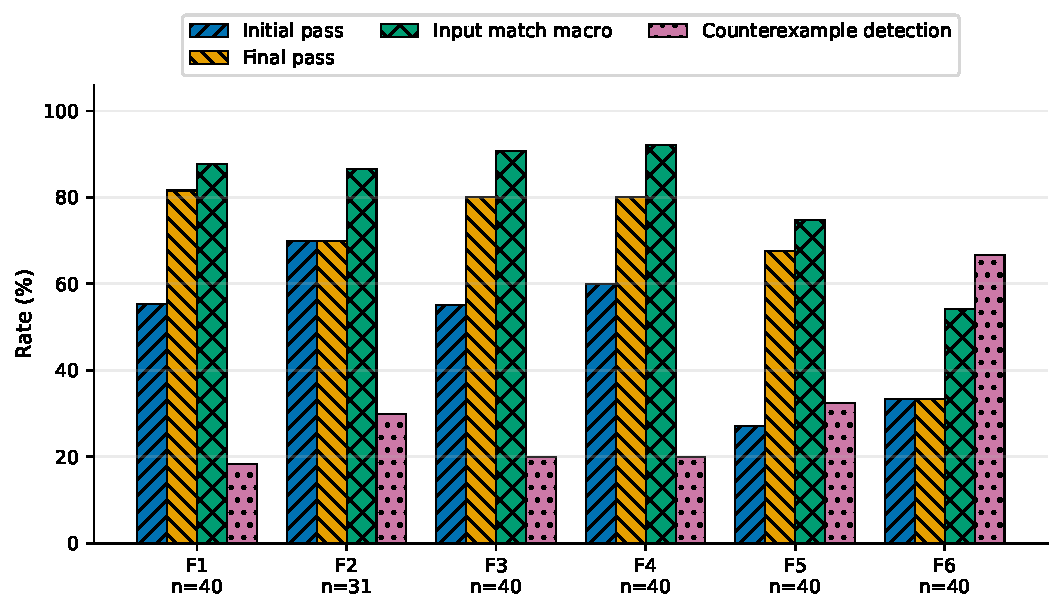
\includegraphics[width=.9\linewidth]{figures/behavioral_performance.pdf}\caption{Behavioral outcomes over conclusive campaigns.}\end{figure}
\begin{figure}[p]\centering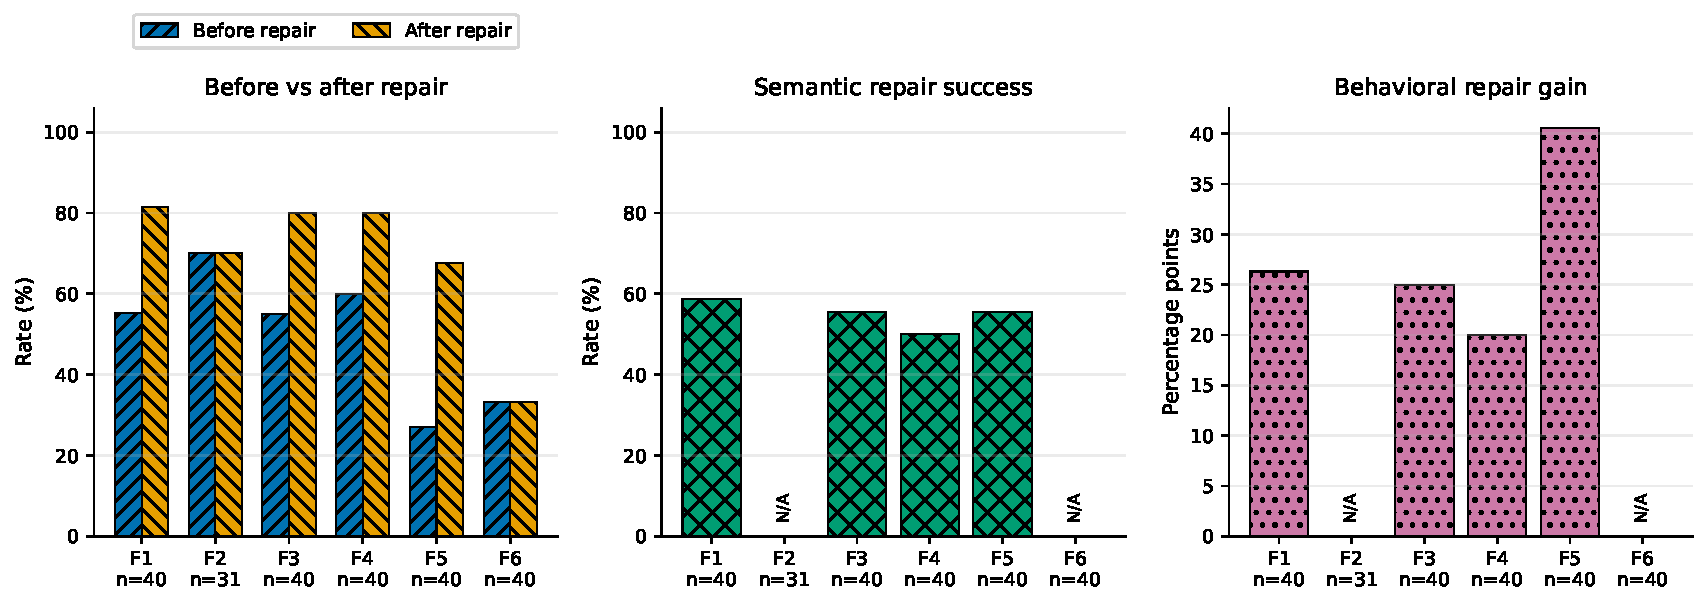
\includegraphics[width=.9\linewidth]{figures/repair_effectiveness.pdf}\caption{Behavioral repair effectiveness; F2, F6 repair fields are N/A.}\end{figure}
\begin{figure}[p]\centering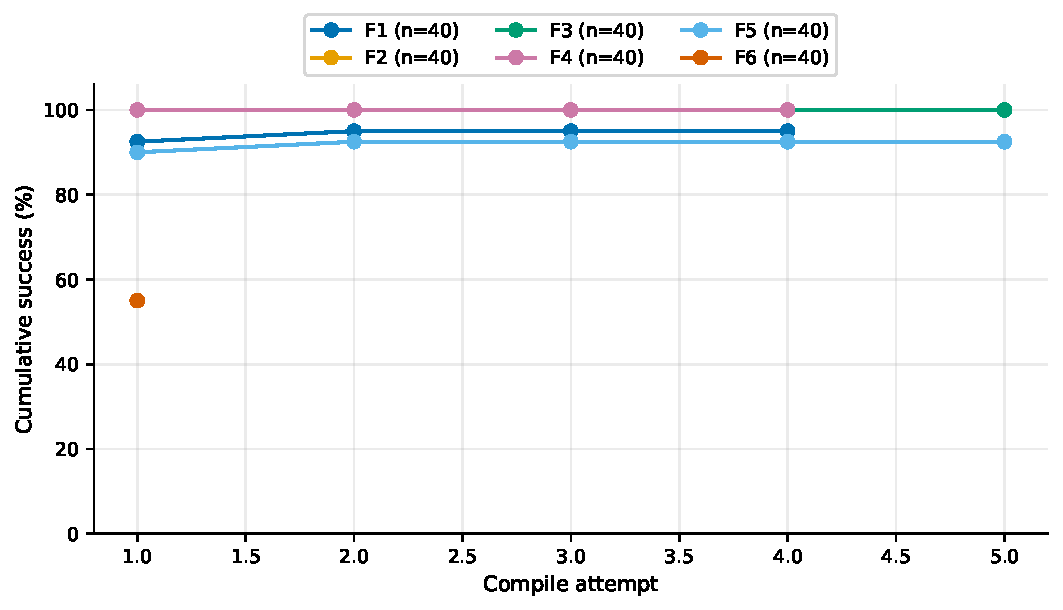
\includegraphics[width=.9\linewidth]{figures/cumulative_compile_success_by_round.pdf}\caption{Cumulative executable creation by compile attempt.}\end{figure}
\begin{figure}[p]\centering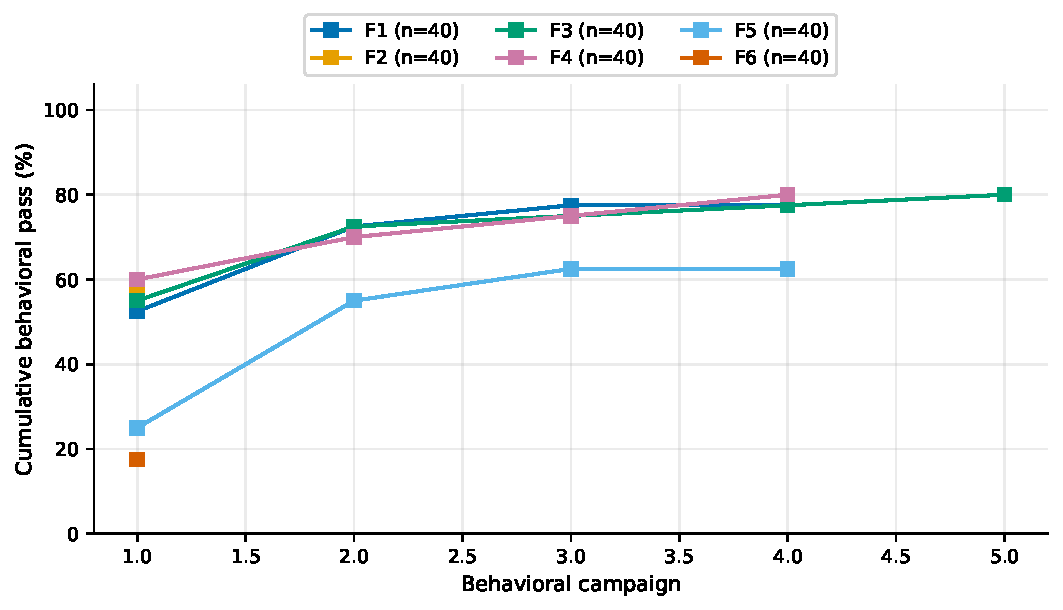
\includegraphics[width=.9\linewidth]{figures/cumulative_behavioral_success_by_round.pdf}\caption{Cumulative behavioral pass by campaign.}\end{figure}
\begin{figure}[p]\centering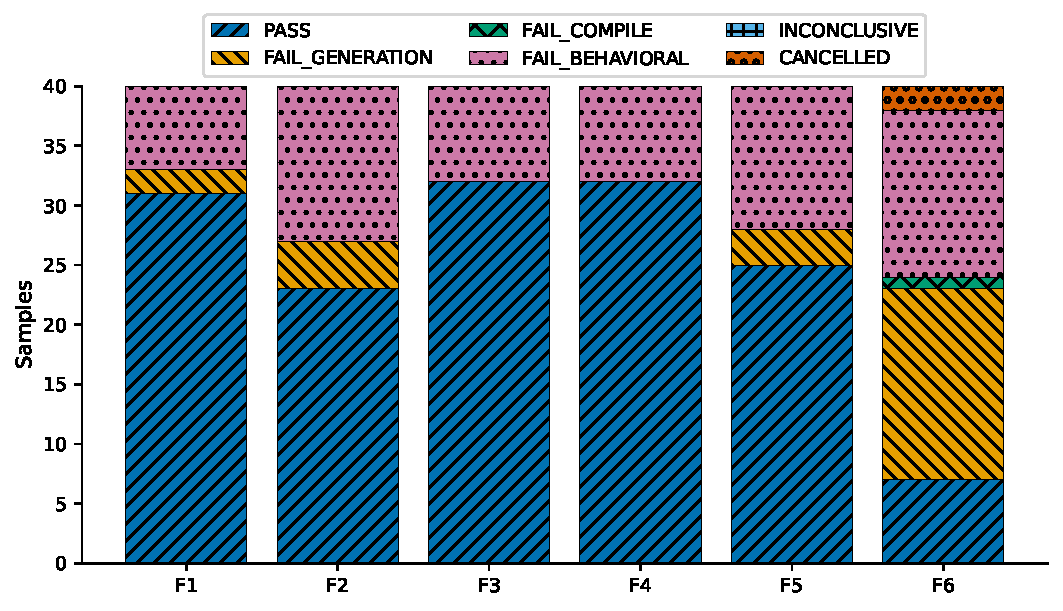
\includegraphics[width=.9\linewidth]{figures/final_status_breakdown.pdf}\caption{Final status distribution without collapsing INCONCLUSIVE into failure.}\end{figure}
\begin{figure}[p]\centering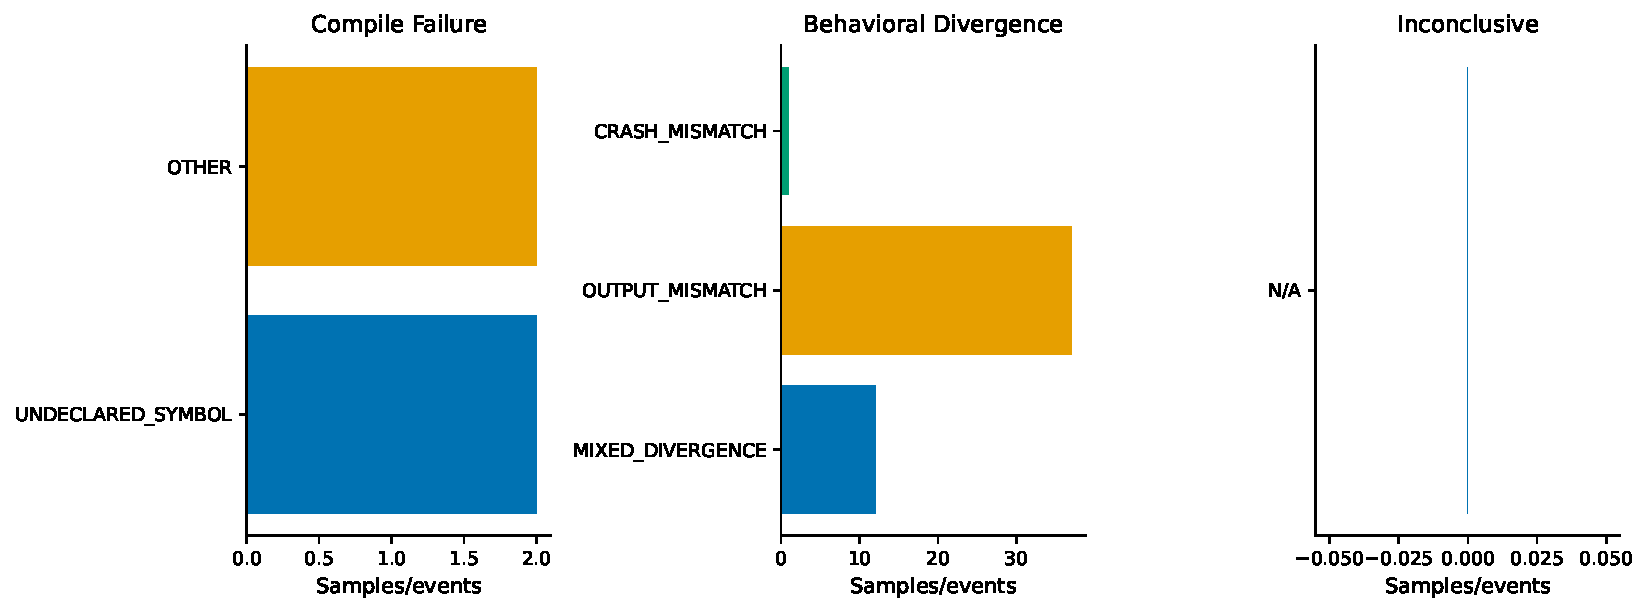
\includegraphics[width=.9\linewidth]{figures/failure_taxonomy.pdf}\caption{Compilation, behavioral, and inconclusive taxonomies.}\end{figure}
\begin{figure}[p]\centering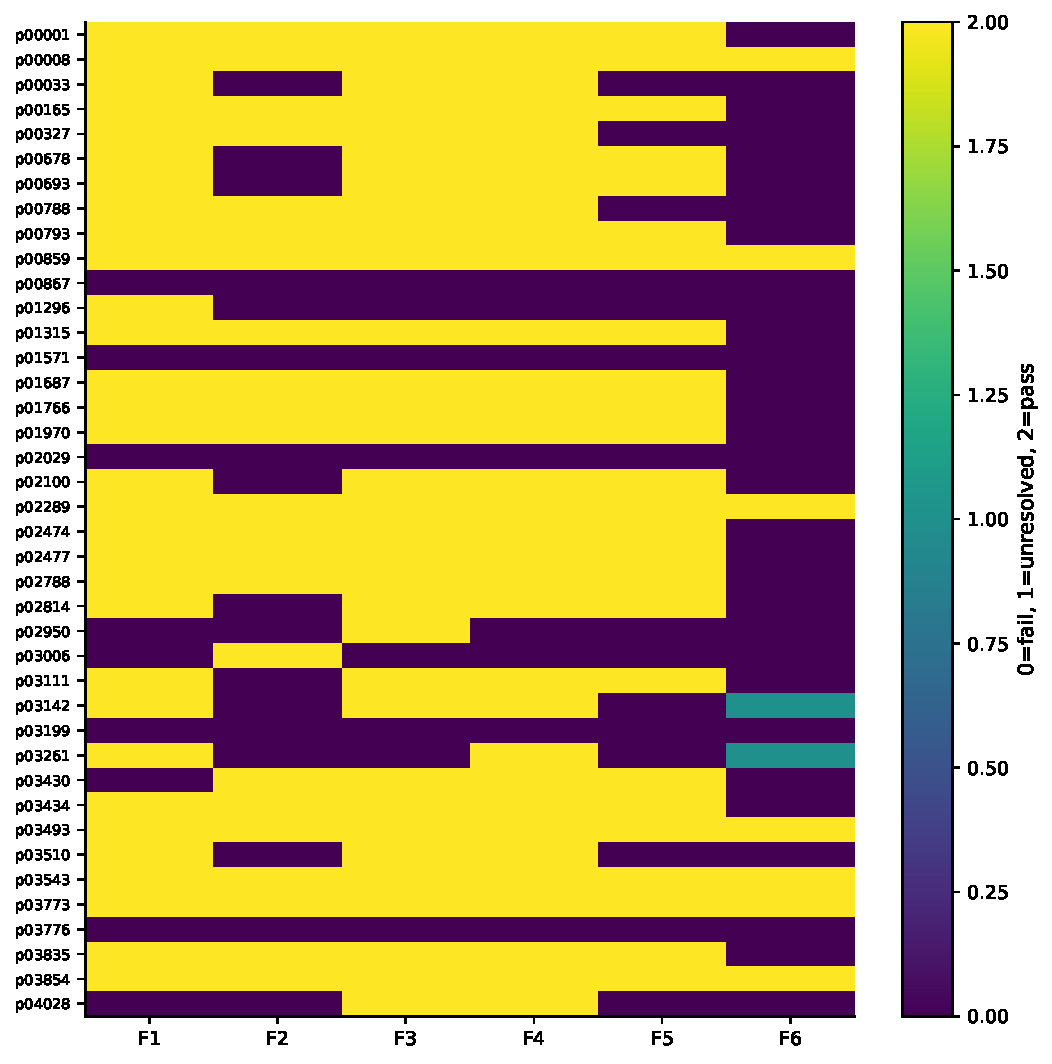
\includegraphics[width=.9\linewidth]{figures/sample_flow_status_heatmap.pdf}\caption{0=fail, 1=unresolved, 2=pass by paired sample and flow.}\end{figure}
\begin{figure}[p]\centering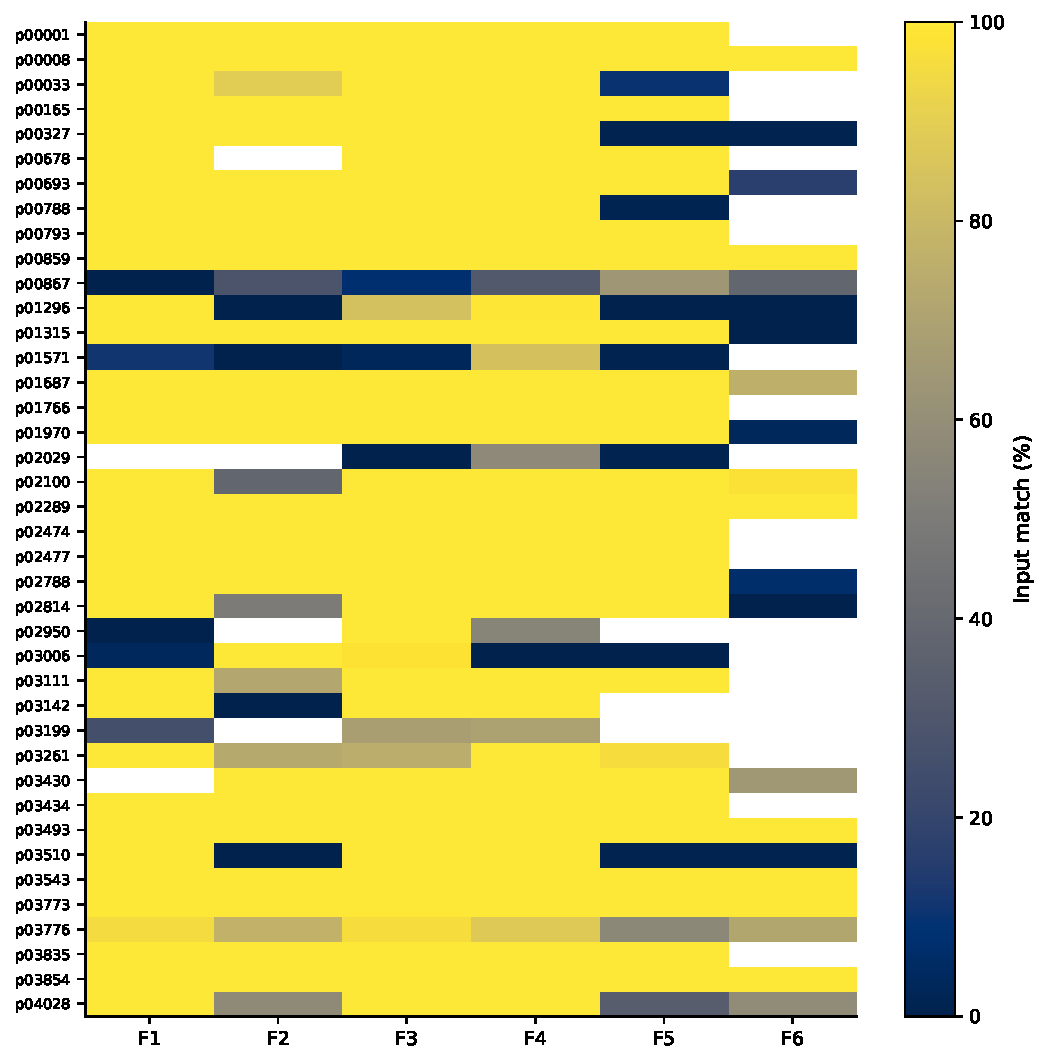
\includegraphics[width=.9\linewidth]{figures/sample_flow_match_heatmap.pdf}\caption{Input match (\%) by paired sample and flow.}\end{figure}
\begin{figure}[p]\centering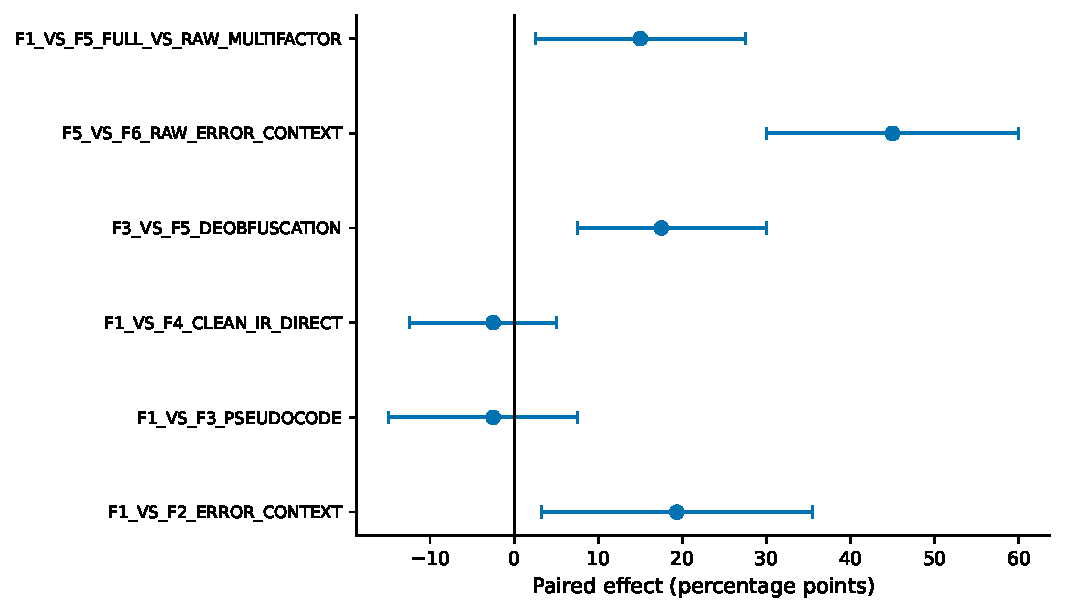
\includegraphics[width=.9\linewidth]{figures/ablation_forest_plot.pdf}\caption{Paired Canonical E2E effects with bootstrap 95\% CI.}\end{figure}
\begin{figure}[p]\centering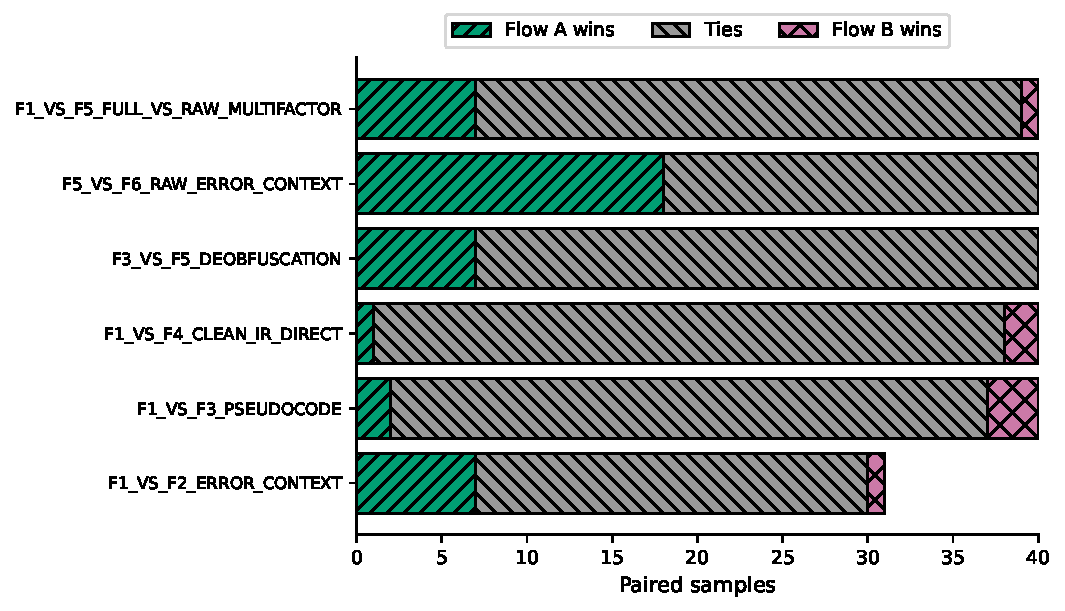
\includegraphics[width=.9\linewidth]{figures/ablation_win_tie_loss.pdf}\caption{Paired win/tie/loss counts for Canonical E2E.}\end{figure}
\begin{figure}[p]\centering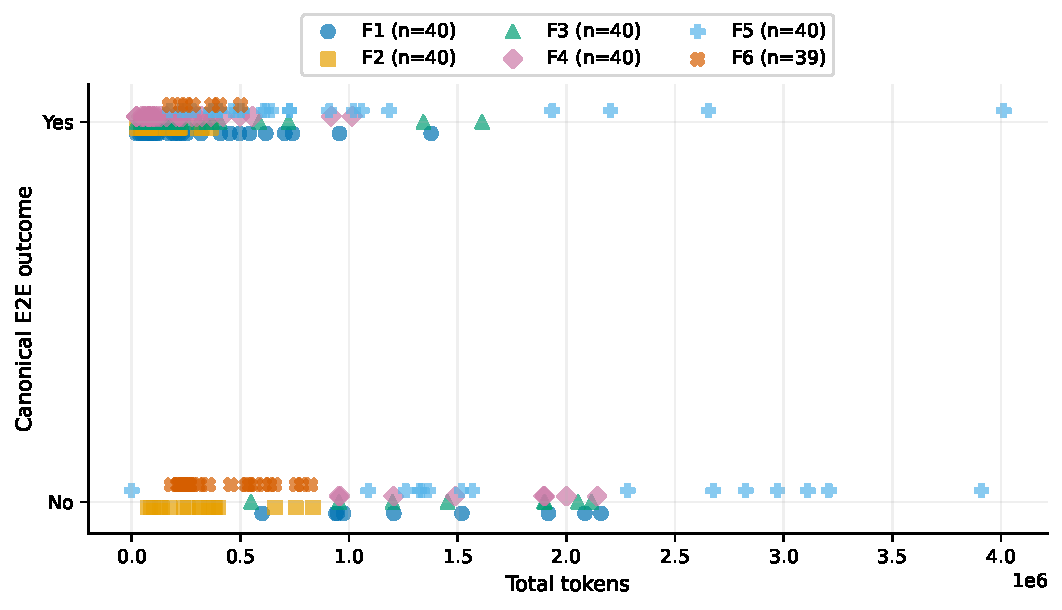
\includegraphics[width=.9\linewidth]{figures/tokens_vs_e2e.pdf}\caption{Total tokens versus Canonical E2E outcome.}\end{figure}
\begin{figure}[p]\centering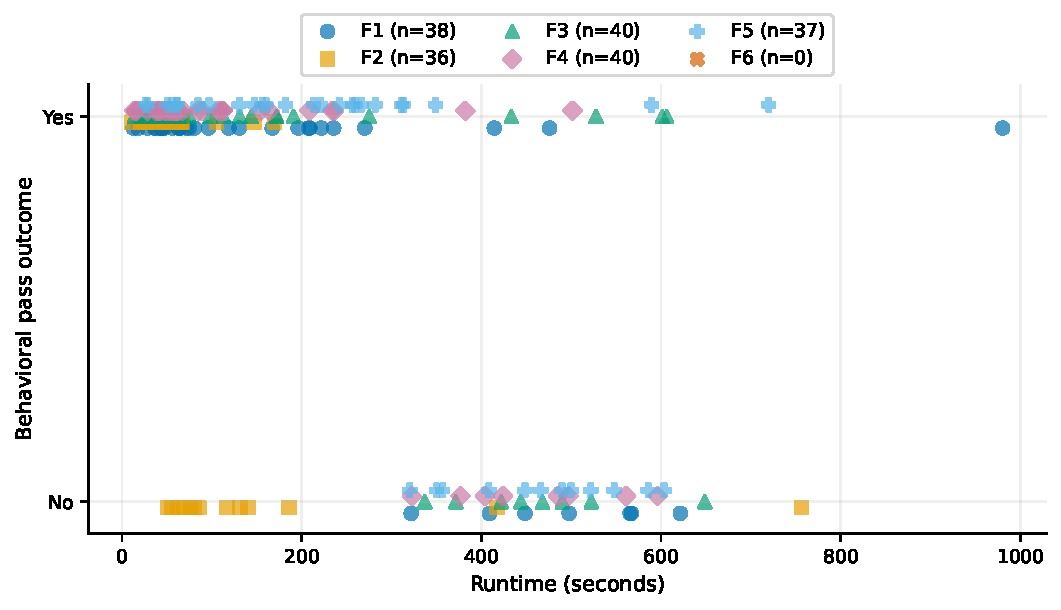
\includegraphics[width=.9\linewidth]{figures/runtime_vs_behavioral_pass.pdf}\caption{Runtime (seconds) versus Behavioral pass outcome.}\end{figure}
\begin{figure}[p]\centering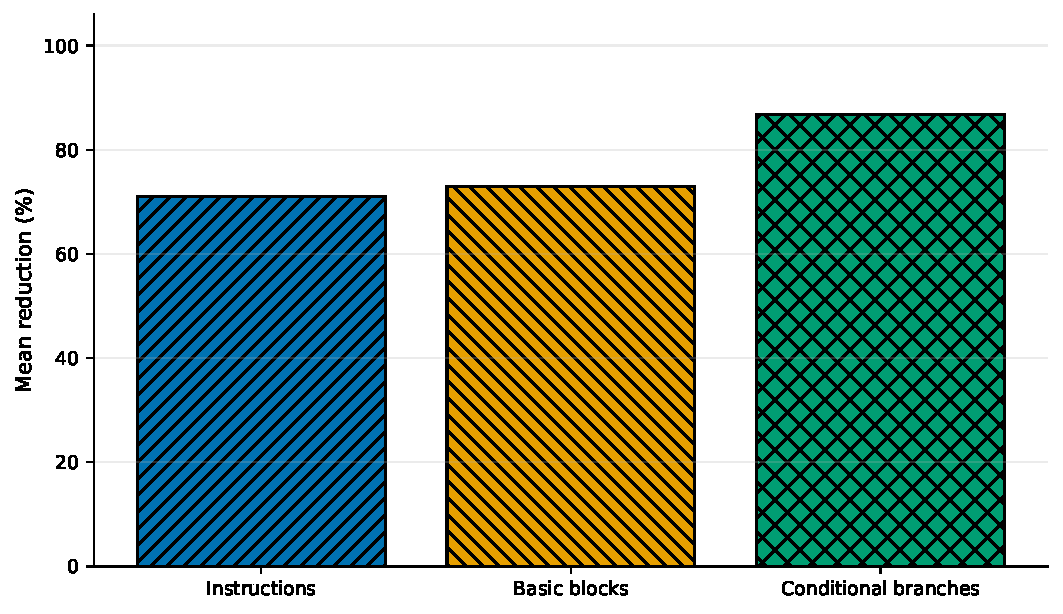
\includegraphics[width=.9\linewidth]{figures/llvm_reduction_summary.pdf}\caption{LLVM simplification metrics; these are not correctness claims.}\end{figure}
\begin{figure}[p]\centering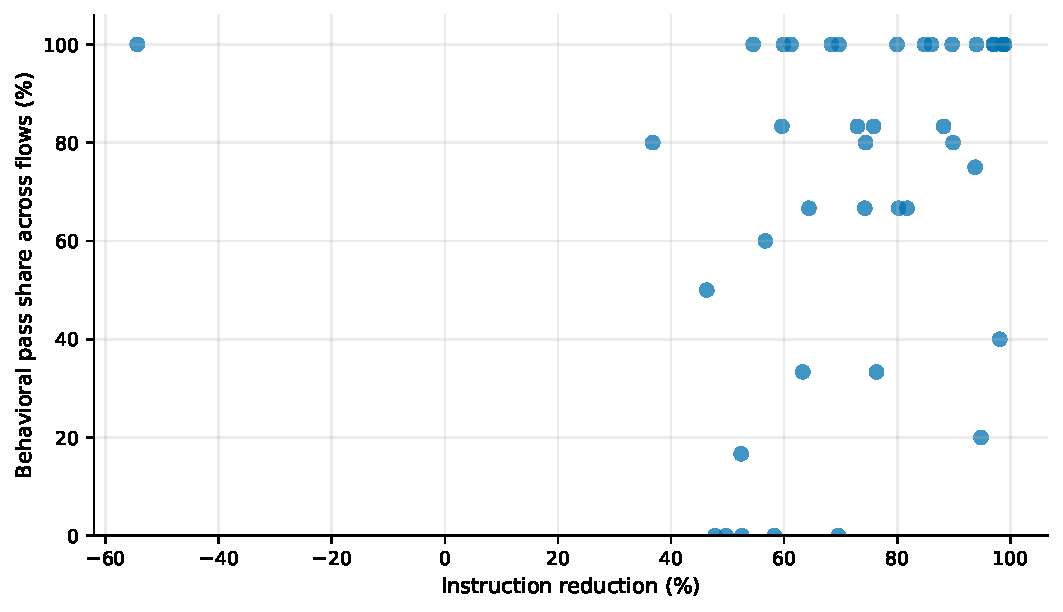
\includegraphics[width=.9\linewidth]{figures/llvm_reduction_vs_behavior.pdf}\caption{Association view only; LLVM reduction is not a semantic oracle.}\end{figure}
\begin{figure}[p]\centering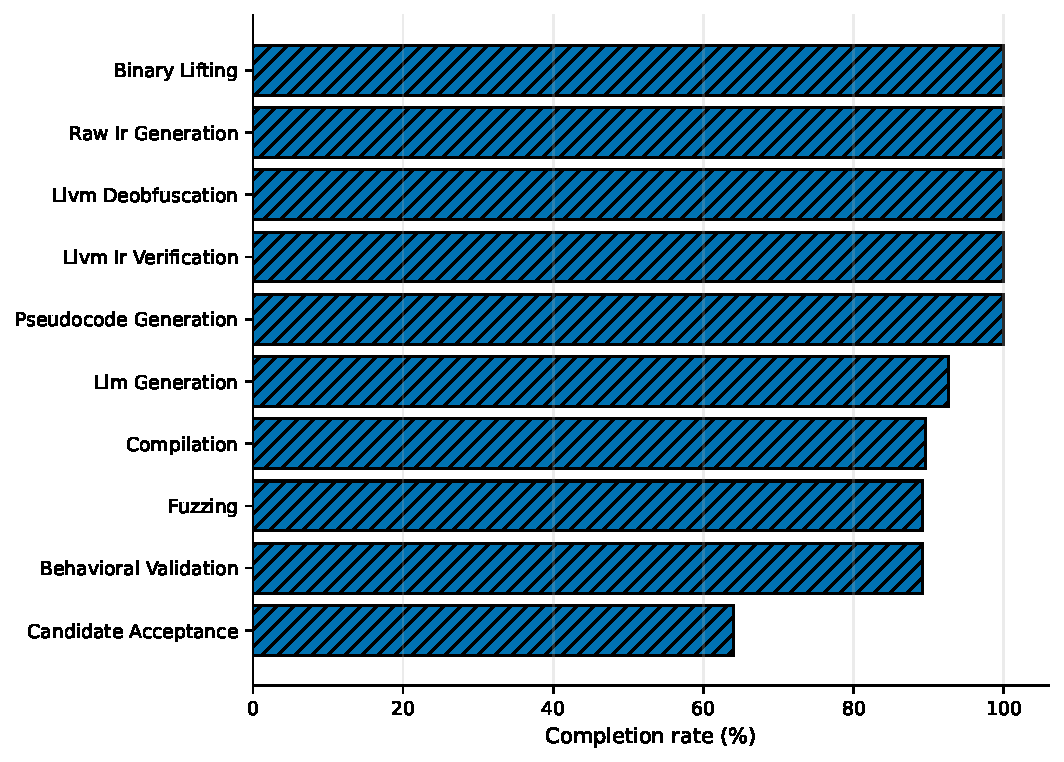
\includegraphics[width=.9\linewidth]{figures/stage_completion_funnel.pdf}\caption{Stage completion rates with explicit numerators and denominators in the report.}\end{figure}
\end{document}
